\chapter{Traffic scheduling}
\label{chap:gf}
%trosku este prepisat tento uvod
One of the pieces of puzzle that make the Internet and generally packet-switched networks work is traffic scheduling. It lies between the second and the~third layer of OSI (or the TCP/IP). That means its turn comes after the network layer does its job: it determined the packet's next hop and particularly the link, through which the device is going to transmit the packet. Before the device hands it over to the data link layer and actually sends it, it waits in a buffer. The buffer is needed because of asynchronism of packet-switched networks (further reasons why buffers are needed are discussed in \autoref{chap:bb}). 

As the Internet grows, more and more different traffic flows through and more pressure is put on maintaining acceptable quality of service QoS. Ever-rising number of services are now provided through internet protocol, that require certain standards: IPTV, VoIP, teleconferencing. % The Internet consist of countless protocols, principles, ideas and algorithms. None of them are perfect, and perfecting any piece of puzzle may have far-reaching consequences.

%When people buy internet access, we pay for certain bandwidth, which Internet service provider (ISP) is obligated to guarantee. However, "internet speed" is not the only factor affecting our day-to-day experience. Great example is web browsing. Size of (most polite) web pages is negligible compared to bandwidth of today's connections. Still, it can take up to seconds to load a page, due to poor quality of service.
%lepsi priklad^^

The term quality of service is used to denote overall performance of the Internet service. Various measurements may be required for different services. Voice over Internet Protocol (VoIP), which enables us to phone each other over the IP, requires small delay, packet loss and jitter. Internet protocol television (IPTV) additionally requires sufficient throughput. On the other hand, e-mail does have little requirements whatsoever. Here are some examples of measurements that affect quality of service:
\begin{itemize}
	\item Throughput --- the bit rate --- number of bits that can be transmitted per second
	\item Packet loss --- ratio of packets, that never reach their destination to all packets.
	\item Packer errors --- packet error happens, when the delivered packet is different than the sent packet.
	\item Delay --- time that elapses between packet sending and receiving.
	\item Jitter --- variance in delay of consecutive packets.
\end{itemize}

The natural simplest solution is to implement first-come first-serve (FCFS) queue. However, as shown throughout this chapter, problems arise, that can be solved by using more sophisticated methods instead.

There is wide range of requirements ideal traffic scheduler should satisfy. It starts with avoiding poor performance, and other negative phenomena observed in networks, continues with enforcing fairness for all applications (users). Internet service providers use scheduling to define the shape of traffic provided to customers. Researchers have realised the potential years ago and this chapter offers a summary of basic concepts used in the area.


%connection-oriented vs connectionless networks - connectionless are prone to statistical variations (bursts), while in connection-oriented it is easier to allocate the right amount of resources as the connection is began.





\section{Bufferbloat}
\label{chap:bb}

In gateways of packet-switched networks, short-term differences between arrival and departure rate naturally happen. To balance these bursts, gateways use buffers --- packets wait in queues until they can be sent towards their destination. This helps avoiding outgoing link starvation and increases throughput. Without buffers, the gateway has no place to store incoming packets and they get dropped, which decrease throughput.


However, the more packets are in a queue, the longer packets stay in it and the longer it takes to be delivered. Unfortunately, queues in modern networks tend to fill up and stay 'bloated' \cite{Gettys:2012:BDB:2063176.2063196}. That means some amount of packets always stay in the queue (it never becomes empty), even if there are no incoming bursts to balance.

\begin{figure}
	\centering
	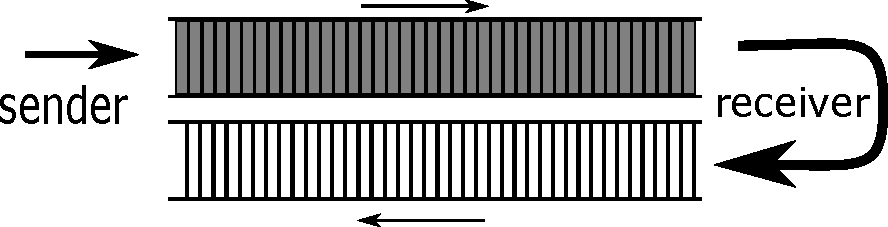
\includegraphics[width=137mm]{drawings/tcp_no_bottleneck}
	\caption{TCP without bottleneck. The grey rectangles are packets. Horizontal dimension is time, vertical is bandwidth. That means the area of rectangle is size of packet.}
	\label{fig01:no_bottle}
\end{figure}

To understand why queues become bloated, let's take a look at Transport Control Protocol (TCP), which is the most widely used layer 4 protocol. It achieves its reliability with the following policy: After a packet is transmitted, the receiver sends an ACK packet back to sender, to let him know which packets were successfully received, and which packets must the sender resend. But waiting on ACK after each packet would provide miserable throughput and most of the time both sides would wait for single packet. Instead, the sender goes ahead and transmit packets without getting ACKs on previous ones. This fills the whole route, so at all times one packet is being sent, and one packet is being received. The ACKs that come back retain the same spacing. The situation is displayed in Figure \ref{fig01:no_bottle}.

Figure \ref{fig01:no_bottle} shows connection with constant bandwidth along whole path, which is rarely the case in today's Internet. Typical path between the communicants consists of many hops with links of different bandwidth. That means somewhere must be a bottleneck - a link with lowest bandwidth. If the sender transmitted at the rate of the adjacent link, the network would become congested. The bottleneck link would not be able to forward all the incoming traffic, its buffer would fill, and the rest of the arriving packets would be dropped. That actually induces even more traffic, because sender would try to resend the dropped packets.


%tcp by potrebovalo vediet aky badwidth ma bottleneck
TCP must limit the upstream rate. In ideal case, it would work at the rate of the slowest link. However, the sender does not have any information about bottleneck whatsoever. Thus, TCP uses congestion window: it is amount of bytes TCP can send without receiving an ACK. When an ACK is received, it frees space in congestion window, and TCP may permit sending the next packet, filling the window again. The sender receives the first ACK after round trip time (RTT) - the time it takes to transmit a packet through path sender-receiver-sender.

To maximize throughput, size of congestion window should be at least the (bottleneck) bandwidth-delay product (product of bandwidth and RTT) bytes. In this case, the sender fills the pipe with packets just before it receives the first ACK and is allowed to send the following packets. On the other hand, if the congestion window exceeds the bandwidth-delay product, the excessive packets stay in queues along the path and cause delay. 

%TCP uses slow start algorithm to find ideal congestion window at start, and then congestion control algorithm takes over to maintain it near the inflection point of maximized throughput and minimizing delay. This if solution to avoiding congestion collapse, but the Internet encounters problem of persistently full buffers - bufferbloat.



Bufferbloat is caused by mismatch between congestion window and actual RTT \cite{CoDel}. In reality, estimating the window size is difficult. Always-changing network load affect both RTT and bandwidth, paths change thanks to rerouteing. Buffers can really only be measured at the bottleneck and even there it is hard to differentiate between useful and useless buffers that only cause delay.

\begin{figure}
	\centering
	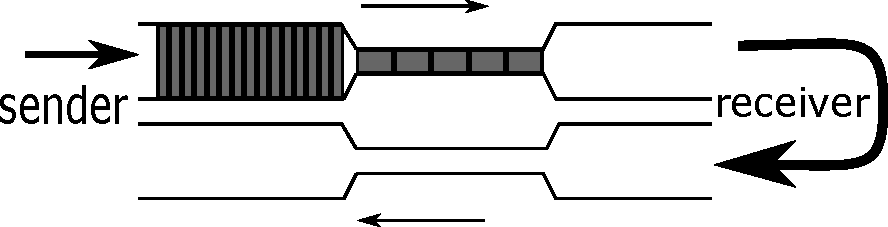
\includegraphics[width=137mm]{drawings/tcp_bottleneck_1}
	\caption{Start of a TCP communication.}
	
	\label{fig02:bottle_1}
\end{figure}


Figure \ref{fig02:bottle_1} shows a starting TCP communication. The illustrated network consists of 3 subnetworks. The left and the right have bandwidth 30 Mb/s, the middle one has 10 Mb/s. One packet has 30kb. The TCP Congestion window is 20 packets. The sender starts by transmitting whole window of packets back to back. They arrive at edge of the bottleneck network and get enqueued there, because of the bandwidth difference between left and middle subnetworks. A packet arrives from the left network every 1 ms, but only every 3 ms is one dequeued. At the right side, they retain spacing given by bottleneck as shown in Figure \ref{fig03:bottle_2}. The receiver turns incoming packets into ACKs with the same spacing. The sender then sends one packet of data for each ACK it gets.

This way, after one RTT, the whole connection gets into state of equilibrium. The bottleneck is fully utilized, so the throughput is as high as possible. However, the queue at the middle network never gets empty. At first, it has to hold the burst of the whole congestion window. Once all 20 packets are sent, 14 of them are waiting in the queue, 6 are already forwarded towards the middle network. Then, no packets are enqueued, and every 3 ms one is dequeued. Until one RTT passes, first ACK is delivered, and next packet is sent into left network. After that, one packet arrives and one leaves every 3 ms. 5 packets stay there and every one of them waits long 15 milliseconds. Also, they block buffer space other connections could use. 

\begin{figure}
	\centering
	\includegraphics[width=137mm]{drawings/tcp_bottleneck_2}
	\caption{TCP after one RTT}
	
	\label{fig03:bottle_2}
\end{figure}

The reason, why the packets stay in the buffer in Figure \ref{fig03:bottle_2} is, that the congestion window is set to 5 more packets than the bandwidth-delay product. Determining the size of the congestion window is not an easy task. At start of TCP, slow start algorithm \cite{Jacobson:1988:CAC:52324.52356} is used to determine the size of congestion window. It grows exponentially, increasing size of the window with each ACK received, until a threshold is reached or a packet is dropped. After that, congestion avoidance takes over to maintain it. Over the years of TCP in service, many variants were introduced. Currently, CUBIC \cite{CUBIC} is used widely. 

%emhasize that it is a way to communicate
The congestion windows are managed by the TCP endpoints, while congestion and bufferbloat takes place in gateways along the path. There is no direct communication channel between them. When the buffer becomes full, the next packets must be dropped simply because there is no room for them. When TCP does not receive an ACK, it the congestion avoidance algorithm reduces the window and slows down.

Explicit Congesion Notification (ECN) \cite{rfc3168:ECN} is relatively new protocol. There are 2 bits reserved for ECN in the IP header, so packets may be marked, that there is ongoing congestion. Both sides have to support ECN  - the receiver has to read the 2 bits and send ACK with the same bits back. The sender then may react like the ACK does not arrive at all. In May 2017, 70 \% of popular websites provided passive support for ECN\cite{ECN:proceedings}.

This all indicated, that simple tail drop queues, which drop packets only when they are full may be superseded by more sophisticated queues right in the gateways. It involves the counter-intuitive idea of dropping perfectly good packets even if buffer is not full yet. But the drop indicates a problem, while still having room for balancing bursts. This approach is called Active Queue Management (AQM), and is recommended to use throughout the Internet.


\subsection{Random Early Detection}

\begin{figure}
	\centering
	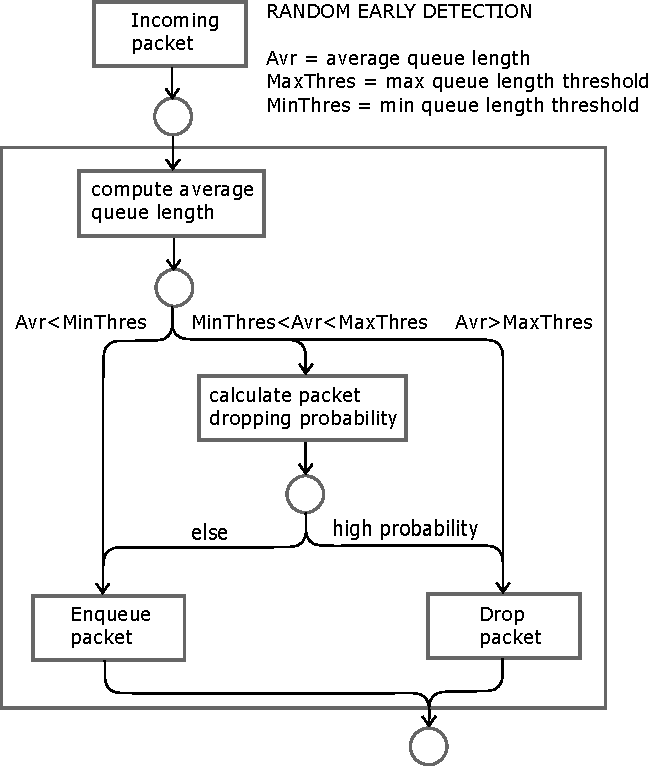
\includegraphics[width=137mm]{drawings/RED}
	\caption{The Random Early Drop algorithm  (Image taken from wikipedia \cite{RED:picture}) }
	
	\label{fig04:RED}
\end{figure}

%o TCP sychronization hovorim prvy krat az tu

In 1993, Sally Floyd and Van Jacobson introduced Random Early Drop (RED) \cite{Floyd:1993:RED:169931.169935}. It monitored the average length of queue. Based on the average, it may drop (mark) incoming packet with certain (possibly 100 \%) probability, which is function of average. It addressed congestion avoidance problem as well as TCP synchronization problem, that were encountered using tail drop. However, it had quite a few parameters, which have to be set differently in various networks. Without this tuning, it functioned poorly, which led to general reluctance of deployment, although it was recommended by Internet Engineering Task Force \cite{rfc2309} in 1998.

To determine the average, RED uses exponential weighted moving average:
\[
avg := (1 - w_q)avg+w_qq.
\]
$q$ is number of packets in the queue and $w_q$ is parameter of RED that represents degree of weighting decrease, or how much the average responds to new packets and how much weight have the past states. Too high $w_q$ would mean bias against short bursts. With lower $w_q$, the average is more fluid and queue responds to congestion slower.

At each enqueue, the $avg$ is compared to two parameters $min_{th}$ and $max_{th}$, as shows Figure \ref{fig04:RED}. If it is lower than $min_{th}$, packet is just enqueued as is. If $avg$ is higher than $max_{th}$, the packet is marked (dropped). This ensures that if endpoints respond to the marking properly, or packets are actually dropped, the number of packets in queue will not exceed the maximum for long.

If $avg$ is between the thresholds $min_{th}$ and $max_{th}$, the packet is marked (dropped) with probability $p_a$, that is function of the average and number of packets since the last drop. Let $p_b$ be linear function of $avg$ that varies from 0 to $max_p$ ($max_p$ is parameter of RED):
\[
  p_b = max_p \frac{(avg - min_{th})}{max_{th} - min_{th}}.
\]
Further, the final marking probability $p_a$ depends on when was the last packet marked (dropped):
\[
p_a = \frac{p_b}{1-count \cdot p_b},
\]
where $count$ is number of packets that were enqueued since the last mark (drop). This ensures, that dropped packets will never be too far, nor too close to each other\cite[Section 7]{Floyd:1993:RED:169931.169935}.

RED has also the option to work based on number of bytes in the buffer instead the number of packets. In this case:
\[
  p_b = max_p \frac{(avg - min_{th})}{max_{th} - min_{th}}
\]\[
  p_b = p_b \frac{size_{packet}}{size_{max}}
\]\[
  p_a = \frac{p_b}{1-count \cdot p_b},
\]
where $size_{packet}$ is size of the packet being enqueued and $size_{max}$ is maximum size of packet. This way, large packets are more likely to get marked, and the probability corresponds more precisely to actual time that the packets spend in the queue.

%!!!!!!!!!!!!!!!!!!je v pohode tam dat takyto odstavec o ktorom neviem vela??
Over the years, several variants of RED have been introduced. With Weighted RED, different packets have different probability functions for different classes of traffic (classified for example by DSCP). Adaptive RED \cite{Floyd01adaptivered:} tunes the RED algorithm to remove sensitivity to some of the parameters. Robust RED \cite{RRED} was proposed to counter low-rate Denial-of-Service attacks.

\subsection{CoDel}
\label{CoDel}
In 2012, Jacobson and Nichols introduced Controlled Delay (CoDel) algorithm \cite{CoDel}. Their AQM uses local minimum length of queue as indication of bufferbloat. Additionally, it works only with sojourn time --- the time packets spend in queue. That means it is independent of bandwidths of adjacent links, because it only works with time --- if it is deployed in a backbone, with 10 Gb/s bandwidth, acceptable queue will be 50 Mb big. On the other hand, on slow links, say 10 Mb/s, corresponding acceptable buffer is only 50 kb. CoDel measures the time packets spend in queue and if it exceeds a threshold for a longer uninterrupted time, it starts to drop packets.

It has 2 parameters:
\begin{itemize}
	\item $Target$ is the target delay CoDel tries to keep. Defaults at 5 ms.
	\item $Interval$ sets period of time for which it is OK to exceed $Target$. Defaults at 100 ms.
\end{itemize}
So CoDel drops packets, if packets spend more than $Target$ time in the queue for more than $Interval$ time. Also, CoDel does not drop packets, if fewer that MTU (Maximum Transmission Unit) worth of bytes is in queue.

Every time a packet arrives, a time stamp is tagged to it. At dequeue, CoDel looks how long was the dequeued packet in the queue. If packets have exceeded the $Target$ time for at least $Interval$, CoDel enters dropping state. In this state, packets are dropped at an increasing rate until the sojourn time of packets at front is lower than $Target$. After each drop, the next drop time is calculated as follows:
\[
  DropInterval = \frac{Interval}{\sqrt{count}},
\]
where count is the number of packets dropped since dropping state entry and DropInterval is the time after the next packet will be dropped.

--- je tu treba nejaky takyto transition? ---
 
CoDel and RED both addressed the bufferbloat problem and both managed to mitigate the problem at the very least. CoDel superseded RED by its easiness to deploy. However, both algorithms work above a single FIFO queue, which is their limitation. The next section shows how traffic scheduling may benefit from using multiple queues in parallel.

\section{Fair queueing}
\label{sec:fair_queueing}
Research shows that simple first-come, first-serve (FCFS) scheduling does not treat all network users fairly in all situations. In many cases, we want to ensure that every user of a network is provided with the same quality of service. Further, it is beneficial if scheduling separates well and ill-behaved users, so that only the latter experience consequences of their behaviour. Set of algorithms that enable this is called fair queueing.

In many of the proposed solutions, fairness is achieved by adding firewalls between different streams of packets traversing network, or flows. We use definition from \cite{Zhang:1990:VCN:99517.99525}. A flow has two properties:
\begin{itemize}
	\item A flow is a stream of packets that traverses the same route from the source to the destination and requires the same grade of service at each router or gateway in the path.
	\item In addition, every packet can be uniquely assigned to a flow using prespecified fields in the packet header.
\end{itemize}
 
\begin{figure}
	\centering
	\includegraphics[width=137mm]{drawings/parking_lot}
	\caption{The parking lot problem.}
	
	\label{fig05:ParkingLot}
\end{figure}

One of the issues addressed by fair queueing is the parking lot problem. Typically, routers accomplish some amount of fairness by giving fair access to traffic coming from different input links. However, this approach is not fair to all flows. Consider network displayed in Figure \ref{fig05:ParkingLot}. Gateway G1 treats both flows F1 and F2 equally, thus both flows occupy half of link G1--G2. G2 does the same, it gives half of the bandwidth to flow 3 and second half to the traffic from link G1--G2. However, from perspective of flows, F1 and F2 have only 1/4 of the bandwidth while F3 has half of the bandwidth. In the outcoming link of G3, situation is the same and F1 only has one 1/8 of the bandwidth. In other words, portion of bandwidth allocated to flow drops exponentially with number of hops it gets through.

Second issue is related to behaviour of the users themselves. In gateways working on FCFS basis, misbehaving user that sends more traffic than others, and does not slow down on packet drops, may actually get bigger portion of bandwidth than well behaving users. Consider a router with several users connected on LAN, one of them is ill-behaved and generates traffic that by itself exceeds routers out--link. The rest of users detect congestion and slow down, resulting in leaving even bigger proportion of the bandwidth to the bad user. Furthermore, delay discussed in section \ref{chap:bb} is shared among all users and if one bloats the buffer, the others experience consequences too.

To battle these problems, Nagle \cite{Nagle:FQ} proposed to use one FCFS queue per one flow encountered by the gateway. At enqueue, router finds the right queue based on the IP header. Queues are dequeued in a round-robin fashion --- the queues take turns in fixed order. There is a list of all queues and at each dequeue gateway transmits the first packet of the first queue in the list. Then, the first queue is taken from the front and put in the back of the list. In other words, at each dequeue, the queue (flow) that was not served for the longest time is chosen (with the exception of brand new queues).

%flow stealing

This solves both of mentioned problems, maintaining separate queue for each flow requires that the gateway to be able to map from flow identifiactor (for example source-destination address pair, ports and protocol may be considered too) to corresponding queue at each dequeue. This can be easily implemented in $O(log n)$, where n is number of queues, however that is not fast enough for simple routers with ever-rising bandwidths. McKenney discusses several possible implementations in \cite[Section 2]{SFQ}.

Nagle's original algorithm has yet another flaw --- it doesn't take packet size into consideration. So if flow A sends only 100B packets, and flow B sends 500B packets, flow B gets five times more bandwidth. To address the flaw,  Demers et al. devised an ideal algorithm called bit-by-bit round-robin (BR) \cite{demers1989analysis}. It simulates that each queue sends one bit at a time in round-robin fashion. Based on this simulation, it computes time $t$ the whole packet would leave its queue. Then, BR inserts the packet in a queue sorted by $t$. Unfortunately, the best known algorithms that insert into sorted queue require $O(log n)$ time, where n is the number of flows (since at most one packet from each flow needs to be in the priority queue at the same time).

Although the Nagle's FQ algorithm was perfected to be truly fair, it requires too much resources. Following algorithms have O(1) complexity, while being only slightly less fair.


\subsection{Stochastic Fairness Queueing}
%aspon jednu figure bud z FQ alebo SFQ?

SFQ was proposed by McKenney \cite{SFQ} to address the inefficiencies of Nagle’s algorithm. It uses hashing to determine the flow each packet belongs to. Although one would normally require one queue for every flow and thus use hashing with chaining, McKenney suggests using considerably less queues and allow collision. This guarantees $O(1)$ queue determination. The disadvantage is that some flows may collide, end up in the same queue, and thus be treated unfairly. However, if the number of queues is sufficiently larger than the number of active flows, probability of unfairness is low. To further beat this disadvantage, SFQ changes the hashing periodically (e.g. every 10 seconds) by varying salt of the hash function.

SFQ services its queues in round-robin fashion, without taking packet lengths into consideration, so it is unfair, if average packet size vary in the flows.

SFQ uses bufferstealing: When there is no more space in the buffer, a packet is dropped from the queue with the highest number of packets instead of dropping packet being enqueued. To implement this in O(1), McKenney suggests bucket sorting technique: there is an array indexed by number of packets. In $i$-th field of the array, there is a list of all queues that contain $i$ packets.

McKenney's scheme is valuable for bufferstealing and stochastic approach, however does nothing about unfairness caused by flows having different size of packets.

\subsection{Deficit round-robin}
\label{DRR}
Deficit round-robin \cite{EffDRR} is an algorithm that extends SFQ and takes packet length into consideration, so every flow gets the same bandwidth in the long term regardless of its packet characteristics. For each queue, it uses deficit counter that counts how many bytes were dequeued from the queue. If a packet can not be sent because it is too big, remaining bytes in the counter transfer to the next round. It still requires only $O(1)$ time for all the operations.

For each flow, DRR needs parameter $Q_i$, where $i$ is flow number. $Q_i$ roughly specifies how many bytes DRR can send from flow $i$. If $Q_i = Q_j$ for all $i$ and $j$, all queues get the same share of the bandwidth, and thus is fair. If $Q_i$ is twice $Q_j$, $i$-th to $j$-th bandwidth will be in ration $2:1$.

Enqueue is done in the SFQ--way: DRR chooses queue based on hash of certain IP header fields. It keeps list of active queues and works in $O(1)$. When the buffer is full, packet is dropped from the fullest queue instead of dropping the incoming one.

The novelty of DRR lies in modified round-robin. There is a state variable $DC_i$ for each flow. The $DC_i$ is set to $Q_i$. At each round, DRR sends at most $DC_i$ bytes. Once sending next packet would break this rule, DRR puts queue  at the back of active queues list and sets $DC_i$ :
\[
  DC_i = DC_i - b_{sent} + Q_i.
\]
$b_{sent}$ is number of bytes sent that round from queue i --- that is subtracted from $DC_i$. Further, DRR replenishes the deficit counter, so it may send packets in the next round. If there are no packets in queue left, it is deactivated instead of putting it in the back.

\begin{algorithm}
	\caption{DRR dequeue}
	\label{alg01:DRR_deq}
	\begin{algorithmic}
		\While{true}
			\State F $\leftarrow$ pop(ActiveQueues);
			\If {empty(F)}
				\State Deactivate(F)
			\ElsIf{F.DC \textgreater~head(F).PacketSize}
				
					\State {F.DC $\leftarrow$ F.DC - head(F).PacketSize}
					\State \Return pop(F)
			\Else \Comment{The packet is bigger than DC}
				\State F.DC $\leftarrow$ F.DC + Q
				\State push(ActiveQueues, F)
			\EndIf
		\EndWhile
	\end{algorithmic}
\end{algorithm}

Although DRR may not send exactly the same amount of bytes each round, it becomes fair (if all $Q_i$ are equal) in several rounds time, because every round, all that remains in $DC_i$ from the previous round transfers to the next. Thus, any unfairness caused by atomicity of packets are smoothed over time.

%analyza??

\subsection{Flow Queue CoDel}

\begin{figure}
	\centering
	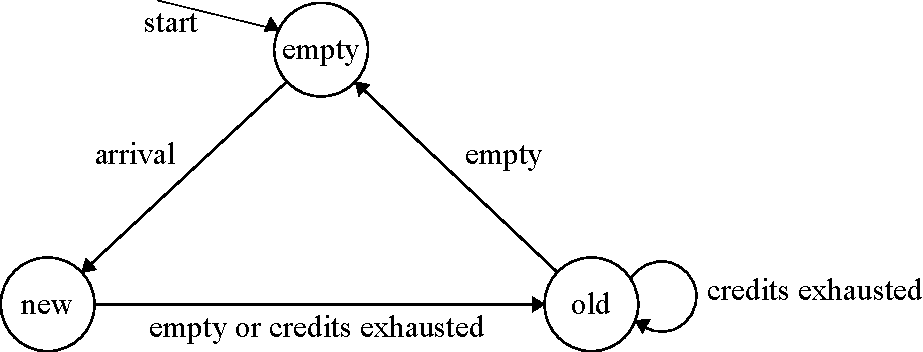
\includegraphics[width=137mm]{drawings/fq_codel}
	\caption{FQ CoDel state-machine}
	
	\label{fig06:fqcodel}
\end{figure}

Flow Queue CoDel \cite{fq_codel} is a traffic scheduler that combines ideas of SFQ and DRR with CoDel bufferbloat battling capability. It uses modified DRR and replaces FCFS queues for flows with CoDel queues. Currently, several linux distributions as well as systemd use FQ CoDel as the default traffic control.

In the context of FQ CoDel, term credits is used instead of deficit counter. However, the two denote the same state variable.

FQ CoDel processes the flows in the DRR fashion, however it divides active queues into two groups: new and old. The new ones are prioritized: packet is never dequeued from an old flow, if list of new queues is not empty. An empty queue becomes new, when a packet is enqueued to it. New queue becomes old (it is pushed at the back of old flows list), if it becomes empty, or its credits ($DC$) are exhausted. An old queue becomes empty, if there are no packets left in it. So every flow has its life cycle in this order: it is first empty, then new, old and empty again. The state machine is illustrated in Figure \ref{fig06:fqcodel}.

FQ CoDel has parameters $Target$ and $Interval$ that configure the underlying CoDels. Further, there is $Quantum$, that is parallel of DRR's $Q_i$, however $Quantum$ applies to all queues. $Limit$ is the maximum number of packets the scheduler can hold at the same time.

When a packet is enqueued in FQ CoDel, its flow is found based on its IP header in the SFQ fashion. Then, CoDel takes it over - it is timestamped and put in the back. If the flow is empty, it is pushed back into the list of new queues and its credits are set to $Quantum$.

To protect buffer from overload, FQ CoDel keeps track of total packets it is holding. Since a packet is just enqueued, $Limit$ may be exceeded. If it is, the algorithm finds queue with the largest byte count and drops 64 packets from the \textit{front}. Dropping several packets at once amortises the time needed to find the longest queue.

The algorithm does most of the work at dequeue. First, it chooses a flow $F$ to dequeue packet from --- either the head of new queues list, or the head of the old queues list, if the new one is empty. If $F$ has negative credits, it means FQ CoDel already served at least $Quantum$ bytes, and pushes it in the back of the old queues list and starts over with choosing $F$.

Second, it dequeues packet from CoDel of flow $F$. Two things may happen:
\begin{enumerate}
	\item CoDel drops all packets on dequeue --- change state of the flow based on Figure \ref{fig06:fqcodel} and start over.
	\item CoDel returns a packet --- subtract the size of packets from credits of flow $F$ and send the packet away.
\end{enumerate}

FQ CoDel is fast and simple enough to be deployed in ordinary home routers. Furthermore, it combines good characteristics of CoDel and SFQ.

\section{Traffic shaping}

In some applications, perfectly fair queueing (the same bandwidth for all) may not be emphasized. Instead, it is beneficial, to give up the best-effort basis in order to maintain good QoS for all users and services in the network, as different services have different needs and different users have different service level agreements. 

Traffic shaping is set of techniques for regulating the average rate and burstiness of a flow of data that enters the network. The customer and ISP agree on certain traffic pattern (or shape) that provider then shall guarantee. ISP tries to suit all application's requirements for QoS. Also, the goal is to describe traffic patterns in a simple and robust way. Traffic shaping provides ISP with the ways to do it. It is also suitable for congestion avoidance, since it controls amount of traffic in network.

%Traffic policing takes care of the opposite aspect of the SLA - limiting the services provided. ISP monitors traffic users generate and if it exceeds the agreed traffic pattern, it may drop packets.

\subsection{Leaky bucket and Token bucket}
\label{token_bucket}
Leaky bucket (first described by Turner in \cite{turner1986new}) and token bucket are two terms used for the same concept, they only use a slightly different analogy with bucket and water/tokens as described in \cite[Section 5.4.2]{Tanenbaum:2002:CN:572404}. However, both schedule packets at constant rate and drop packets, if they flow too fast while allowing certain burstiness.

Both use the same parameters - rate $R$, at which packets leave and size of bucket $B$, also called burst size.

\begin{figure}
	\centering
	\begin{subfigure}{.6\linewidth}
		\centering
		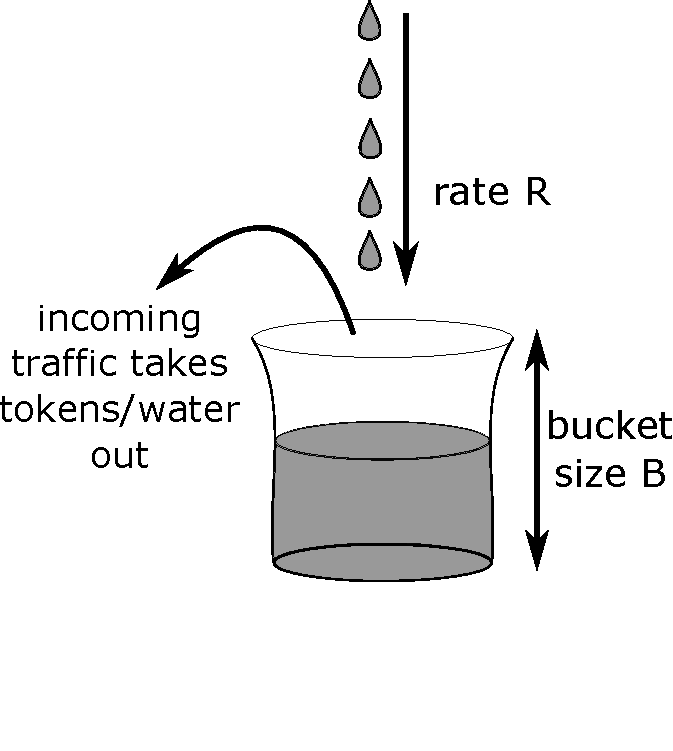
\includegraphics[width=75mm]{drawings/token_bucket}
		\caption{Token bucket}
		\label{fig08:token}
	\end{subfigure}%
	\begin{subfigure}{.4\linewidth}
		\centering
		\includegraphics[width=47mm]{drawings/leaky_bucket}
		\caption{Leaky bucket}
		\label{fig08:leaky}
	\end{subfigure}
	\caption{}
	\label{fig08:token_leaky}
\end{figure}

Illustration of a leaky bucket is in Figure \ref{fig08:leaky}.The algorithm needs a counter variable $C$. If there is any water in the bucket ($C > 0$), it leaks ($C$ decreases) at rate $R$. Every time a packet comes, its size is added to this counter. If $C + PacketSize$ is more than $B$, packet must wait until $C + PacketSize < B$ holds (until enough water leaks) or is dropped. Note, that R is not the same as the output bandwidth. When the bucket is empty, the leaky bucket sends packets as they come until the bucket is filled. 

Token bucket is in Figure \ref{fig08:token}. In this case, algorithm adds tokens to $C$ at rate $R$. Every time a packet passes, it takes tokens equal to its size from the bucket (its packet size is subtracted from $C$), or, if $C - PacketSize < 0$, the packet must wait until enough tokens are in $C$. 

%The general concept is, that there is one bucket for each user.
The concept may be used in two ways --- in the place of scheduler, that actually holds the packets in FCFS queue. Secondly, ISPs can use it in traffic policing, to enforce service level agreement. In that case, token/leaky bucket just manages the buckets based on packets that flow by, and drops them if the buckets are empty/full.

The fundamental feature of the bucket concept is, that it enforces certain bandwidth, while allowing short-term bursts (that are necessary in networks). Let M be maximum output rate in B/s, and t the time between start of burst and dropping (withholding) first packet. Then it holds:
\[
	B + RS = MS,
\]
since water leaks from the bucket even after the burst begins. $B + RS$ is number of bytes bucket permits, $MS$ is the number of bytes output link is able transmit. Thus,
\[
	MaxBurstSize = MS = M\frac{B}{M - R}.
\]

\begin{figure}
	\centering
	\includegraphics[width=137mm]{drawings/tbf}
	\caption{Token bucket filter. Picture taken from wikipedia \cite{TBF:picture}}
	
	\label{fig09:tbf}
\end{figure}

\subsection{Token Bucket Filter}
Token Bucket Filter (TBF) is traffic scheduler implemented in the Linux kernel. It uses the token bucket with FCFS queue. Additionally, it limits peak maximum output rate by adding second small bucket. This bucket is only the size of the maximum transmission unit (MTU), and has the higher configurable peak rate --- TBF never transmits at higher rate that this peak. It prevents the scheduler from taking all the bandwidth of the output link.

It is shown in Figure \ref{fig09:tbf}. TBF enqueues packets into common FCFS queue. It may become full, if number of bytes in it exceeds $Limit$ --- then incoming packet is simply dropped. The dequeue is controlled by two token buckets --- both of them must have enough tokens to allow packet sending. The smaller bucket is size of MTU, $Rate$, $PeakRate$ as well as size of the bigger bucket $Burst$ are parameters of the algorithm.

\subsection{Hierarchical token bucket}
\begin{figure}
	\centering
	\includegraphics[width=137mm]{drawings/hierarchy}
	\caption{Traffic pattern organized in a hierarchy.}
	
	\label{fig10:hierarchy}
\end{figure}
In the area of traffic shaping, it is important to be able to precisely define traffic shape, and to have an algorithm that can follow this definition as precisely as possible. Hierarchic definitions are a natural way to do so. One such hierarchy is shown in Figure \ref{fig10:hierarchy}. It shows a link with 45 Mbps of bandwidth. Two organizations: CUNI and CTU share this link. The first one is guaranteed 25 Mbps and the latter 20 Mbps of the bandwidth. Both organizations then define their internal traffic shape they want to have guaranteed.

Every node is guaranteed to receive \textit{at least} the specified rate at all time. We want the link to be utilized as much as possible at all times. For example, when CUNI only transmits 5 Mbps of video traffic, the excess 3 Mbps may be shared with the rest of classes - first with sibling ones, and if whole CUNI does not generate enough traffic, CTU gets more than the guaranteed 20 Mbps.


Secondly, we need an algorithm, that would enforce the hierarchy. One such algorithm is Hierarchical Token Bucket (HTB) [ref??]. It divides traffic into classes that are further hierarchically grouped in a tree. Classes are divided into 8 levels of priority, which affects delay and distribution of excess resources, but not guaranteed rate. At actual dequeue, HTB uses deficit round-robin to serve all classes of the same priority, while conforming to token bucket limitations.

Every node of the tree takes several parameters:
\begin{itemize}
	\item priority --- classes with higher priority are served first. 0 is the highest priority and 8 is the lowest.
	\item rate --- guaranteed rate the class gets.
	\item ceil --- maximum rate the class can get.
	\item burst --- size of the main bucket (see \ref{token_bucket}).
	\item cburst --- size of the ceil (peak) bucket, should be set small, like average size of packet.
\end{itemize}

There are two token buckets in each class, one with size $burst$ and rate $rate$, the second determines maximum rate, has size $cburst$ and rate $ceil$. The main idea of HTB that allows distribution of excess resources is, that child classes can borrow tokens from their parents, if they have exceeded $rate$ (and do not have any tokens left in the main bucket). They are, however, still limited by $ceil$. According to this, classes can be divided into 3 groups. Then:
\begin{itemize}
	\item Green --- Class has enough tokens (does not exceed $rate$)
	\item Yellow --- Class exceeds $rate$, but does not exceed $ceil$. It may borrow from parent class(es).
	\item Red --- Class exceeds $ceil$, and packets must be backlogged until it gets more tokens (either its own or borrowed).
\end{itemize}


When HTB determines which class to dequeue, it chooses the colour of class first. It serves an yellow class only if there are no green ones. Red classes are never served. Green classes are the ones that do not reach the guaranteed rate yet and thus have highest priority. Next, it filters classes based on priority: HTB never chooses class of priority $i$ if any of the priorities $\left\langle0,i\right)$ are available. If there are more classes of the same priority and color, they are served in round-robin fashion using DRR with the quantums of classes set according to the class $rate$. By default, quantum is 1/10 of $rate$. 

The yellow classes may only borrow from its parent, if it is not red. If it is yellow, it results in recursion --- parent has to borrow tokens from grandparent and so on.

In other words, HTB uses the token bucket hierarchy to mark classes with colour and thus prioritize ones, that have not received $rate$. On the second level, it prioritizes classes with higher priority. On the third level, all classes are equal, thus it uses DRR. On the fourth level, there is usually FCFS queue to buffer the withheld packets. However, in the implementation in the Linux kernel, one may assign any qdisc to each class.

%HFSC
%zaver?
